% 文档类型
%DIF LATEXDIFF DIFFERENCE FILE
%DIF DEL example_old.tex   Thu Jul 11 19:19:50 2019
%DIF ADD example_new.tex   Thu Jul 11 20:47:54 2019
\documentclass{article}

% 引入宏包
\usepackage{graphicx}
\usepackage{amsmath,amsfonts}
\usepackage{algorithm, algorithmic}
\usepackage{hyperref}

% 标题、作者等信息
\title{\LaTeX \, Example}
\author{Zhang San}
\date{2019.07}

% 自定义命令
\newcommand{\Prob}{\mathbb{P}}

% 正文
%DIF PREAMBLE EXTENSION ADDED BY LATEXDIFF
%DIF UNDERLINE PREAMBLE %DIF PREAMBLE
\RequirePackage[normalem]{ulem} %DIF PREAMBLE
\RequirePackage{color}\definecolor{RED}{rgb}{1,0,0}\definecolor{BLUE}{rgb}{0,0,1} %DIF PREAMBLE
\providecommand{\DIFaddtex}[1]{{\protect\color{blue}\uwave{#1}}} %DIF PREAMBLE
\providecommand{\DIFdeltex}[1]{{\protect\color{red}\sout{#1}}}                      %DIF PREAMBLE
%DIF SAFE PREAMBLE %DIF PREAMBLE
\providecommand{\DIFaddbegin}{} %DIF PREAMBLE
\providecommand{\DIFaddend}{} %DIF PREAMBLE
\providecommand{\DIFdelbegin}{} %DIF PREAMBLE
\providecommand{\DIFdelend}{} %DIF PREAMBLE
%DIF FLOATSAFE PREAMBLE %DIF PREAMBLE
\providecommand{\DIFaddFL}[1]{\DIFadd{#1}} %DIF PREAMBLE
\providecommand{\DIFdelFL}[1]{\DIFdel{#1}} %DIF PREAMBLE
\providecommand{\DIFaddbeginFL}{} %DIF PREAMBLE
\providecommand{\DIFaddendFL}{} %DIF PREAMBLE
\providecommand{\DIFdelbeginFL}{} %DIF PREAMBLE
\providecommand{\DIFdelendFL}{} %DIF PREAMBLE
%DIF HYPERREF PREAMBLE %DIF PREAMBLE
\providecommand{\DIFadd}[1]{\texorpdfstring{\DIFaddtex{#1}}{#1}} %DIF PREAMBLE
\providecommand{\DIFdel}[1]{\texorpdfstring{\DIFdeltex{#1}}{}} %DIF PREAMBLE
\newcommand{\DIFscaledelfig}{0.5}
%DIF HIGHLIGHTGRAPHICS PREAMBLE %DIF PREAMBLE
\RequirePackage{settobox} %DIF PREAMBLE
\RequirePackage{letltxmacro} %DIF PREAMBLE
\newsavebox{\DIFdelgraphicsbox} %DIF PREAMBLE
\newlength{\DIFdelgraphicswidth} %DIF PREAMBLE
\newlength{\DIFdelgraphicsheight} %DIF PREAMBLE
% store original definition of \includegraphics %DIF PREAMBLE
\LetLtxMacro{\DIFOincludegraphics}{\includegraphics} %DIF PREAMBLE
\newcommand{\DIFaddincludegraphics}[2][]{{\color{blue}\fbox{\DIFOincludegraphics[#1]{#2}}}} %DIF PREAMBLE
\newcommand{\DIFdelincludegraphics}[2][]{% %DIF PREAMBLE
\sbox{\DIFdelgraphicsbox}{\DIFOincludegraphics[#1]{#2}}% %DIF PREAMBLE
\settoboxwidth{\DIFdelgraphicswidth}{\DIFdelgraphicsbox} %DIF PREAMBLE
\settoboxtotalheight{\DIFdelgraphicsheight}{\DIFdelgraphicsbox} %DIF PREAMBLE
\scalebox{\DIFscaledelfig}{% %DIF PREAMBLE
\parbox[b]{\DIFdelgraphicswidth}{\usebox{\DIFdelgraphicsbox}\\[-\baselineskip] \rule{\DIFdelgraphicswidth}{0em}}\llap{\resizebox{\DIFdelgraphicswidth}{\DIFdelgraphicsheight}{% %DIF PREAMBLE
\setlength{\unitlength}{\DIFdelgraphicswidth}% %DIF PREAMBLE
\begin{picture}(1,1)% %DIF PREAMBLE
\thicklines\linethickness{2pt} %DIF PREAMBLE
{\color[rgb]{1,0,0}\put(0,0){\framebox(1,1){}}}% %DIF PREAMBLE
{\color[rgb]{1,0,0}\put(0,0){\line( 1,1){1}}}% %DIF PREAMBLE
{\color[rgb]{1,0,0}\put(0,1){\line(1,-1){1}}}% %DIF PREAMBLE
\end{picture}% %DIF PREAMBLE
}\hspace*{3pt}}} %DIF PREAMBLE
} %DIF PREAMBLE
\LetLtxMacro{\DIFOaddbegin}{\DIFaddbegin} %DIF PREAMBLE
\LetLtxMacro{\DIFOaddend}{\DIFaddend} %DIF PREAMBLE
\LetLtxMacro{\DIFOdelbegin}{\DIFdelbegin} %DIF PREAMBLE
\LetLtxMacro{\DIFOdelend}{\DIFdelend} %DIF PREAMBLE
\DeclareRobustCommand{\DIFaddbegin}{\DIFOaddbegin \let\includegraphics\DIFaddincludegraphics} %DIF PREAMBLE
\DeclareRobustCommand{\DIFaddend}{\DIFOaddend \let\includegraphics\DIFOincludegraphics} %DIF PREAMBLE
\DeclareRobustCommand{\DIFdelbegin}{\DIFOdelbegin \let\includegraphics\DIFdelincludegraphics} %DIF PREAMBLE
\DeclareRobustCommand{\DIFdelend}{\DIFOaddend \let\includegraphics\DIFOincludegraphics} %DIF PREAMBLE
\LetLtxMacro{\DIFOaddbeginFL}{\DIFaddbeginFL} %DIF PREAMBLE
\LetLtxMacro{\DIFOaddendFL}{\DIFaddendFL} %DIF PREAMBLE
\LetLtxMacro{\DIFOdelbeginFL}{\DIFdelbeginFL} %DIF PREAMBLE
\LetLtxMacro{\DIFOdelendFL}{\DIFdelendFL} %DIF PREAMBLE
\DeclareRobustCommand{\DIFaddbeginFL}{\DIFOaddbeginFL \let\includegraphics\DIFaddincludegraphics} %DIF PREAMBLE
\DeclareRobustCommand{\DIFaddendFL}{\DIFOaddendFL \let\includegraphics\DIFOincludegraphics} %DIF PREAMBLE
\DeclareRobustCommand{\DIFdelbeginFL}{\DIFOdelbeginFL \let\includegraphics\DIFdelincludegraphics} %DIF PREAMBLE
\DeclareRobustCommand{\DIFdelendFL}{\DIFOaddendFL \let\includegraphics\DIFOincludegraphics} %DIF PREAMBLE
%DIF END PREAMBLE EXTENSION ADDED BY LATEXDIFF

\begin{document}

\maketitle

\begin{abstract}
This is the abstract. This is the abstract. This is the abstract. This is the abstract. This is the abstract. This is the abstract. This is the abstract. This is the abstract.This is the abstract. This is the abstract. This is the abstract.This is the abstract.This is the abstract.This is the abstract.
\end{abstract}


% 节
\section{Introduction} 

% 小节
\subsection{Background}




\DIFdelbegin \DIFdel{This is a }%DIFDELCMD < \LaTeX %%%
\DIFdel{document.
}%DIFDELCMD < 

%DIFDELCMD < %%%
\DIFdelend \subsection{Math}
\DIFdelbegin %DIFDELCMD < 

%DIFDELCMD < %%%
\DIFdel{This is an }\DIFdelend \DIFaddbegin \DIFadd{Add something.
This is a }\DIFaddend stochastic differential eqation: 
\begin{equation}\label{sde}
\left\{
\begin{aligned}
	dX(t) &= f\big(X(t)\big)dt + \sum_{r=1}^m g_r\big(X(t)\big) \circ dW_r(t), \quad t\in [0, T],\\
	X(0) &= X_0,
\end{aligned}\right.
\end{equation}
where $f(x) \in \mathbb{R}^n$ is called the drift.

\DIFdelbegin \DIFdel{Equation }\DIFdelend \DIFaddbegin \DIFadd{Eq. }\DIFaddend \ref{sde} is an SDE.


\begin{itemize}
	\item First .....
	\begin{itemize}
		\item aaaaa
		\item bbbbb
	\end{itemize}
	\item Second .....
	\item Third ....
\end{itemize}

\begin{enumerate}
	\item First .....
	\item Second .....
	\begin{itemize}
		\item aaaaaaaa
		\item bbbbbbbb
	\end{itemize}
	\item Third ....
\end{enumerate}

\subsection{Figure}

Figure \ref{fig1} is a path of an one dimensional Wiener Process.

\begin{figure}[htbp]
	\centering
	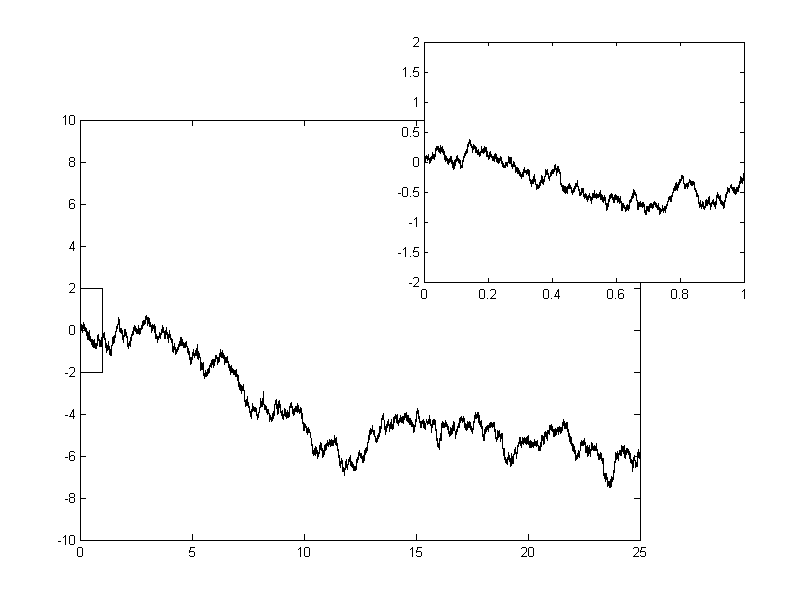
\includegraphics[width=0.7\linewidth]{Wiener_process_zoom}
	\caption{This is the figure caption.}
	\label{fig1}
\end{figure}

\subsubsection{Table}

\begin{table}[htbp]
	\centering
	\begin{tabular}{l|lllll}
		\hline
		A & B & C & D & E  & F \\ \hline
		1 & 2 & 3 & 4 & 5  & 6 \\
		7 & 8 & 9 & 10 & 11 & 12 \\ \hline
	\end{tabular}
	\caption{This is the table caption.}
\end{table}



\subsection{Citation}

This is a citation\cite{Silver2016Mastering,Mnih2015Human,pmlr-v48-mniha16}.


\subsection{Algorithm}

\begin{algorithm}
	\caption{Calculate $y = x^n$}
	\label{alg1}
	\begin{algorithmic}
		\REQUIRE $n \geq 0 \vee x \neq 0$
		\ENSURE $y = x^n$
		\STATE $y \leftarrow 1$
		\IF{$n < 0$}
		\STATE $X \leftarrow 1 / x$
		\STATE $N \leftarrow -n$
		\ELSE
		\STATE $X \leftarrow x$
		\STATE $N \leftarrow n$
		\ENDIF
		\WHILE{$N \neq 0$}
		\IF{$N$ is even}
		\STATE $X \leftarrow X \times X$
		\STATE $N \leftarrow N / 2$
		\ELSE[$N$ is odd]
		\STATE $y \leftarrow y \times X$
		\STATE $N \leftarrow N - 1$
		\ENDIF
		\ENDWHILE
	\end{algorithmic}
\end{algorithm}



% 参考文献样式,根据需要选择
\bibliographystyle{IEEEtran}

% 参考文献文件
\bibliography{references.bib}

\end{document}
